
\section{Ein kurzer geschichtlicher Abriss}
Wir wollen auch einen kurzen Abriss der durchaus interessanten Geschichte der Energieübertragung mit Gleich- und Wechselspannung geben.

Die Geschichte der elektrischen Energie begann 1882 auf der Internationalen Ausstellung in München – mit einer Gleichstrom-Anlage. Der französische Physiker Marcel Deprez übertrug einer elektrische Leistung von 1,4 kW von Miesbach nach München – also über 57 km – mit zwei einfachen Telegrafendrähten mit einer Spannung zwischen 1,5 kV und 2,0 kV. Die Demonstationsanlage betrieb in München die Pumpen eines Springbrunnens. Die Verluste der Anlage betrugen 78\%. Eine weitere Steigerung der Spannung auf 6 kV scheiterte an Isolationsschwierigkeiten beim Gleichstrom-Generator. Diese Problem wurde 1884 von Lafontaine gelöst, indem mehrere von einander isoliert montierte Generatoren parallelgeschalten wurden und auch auf der Verbraucher Seite wurden parallelgeschaltene Motoren verwendet. Dadurch konnte der Wirkungsgrad eine 50 km langen Leitung auch 50\% erhöht und 70 kW übertragen werden.\cite{Schymroch}

Auch nach Entdeckung des Transformators im Jahr darauf, wurde Wechselspannung -- obwohl sie sich Verlustarm hochspannen ließ -- weiterhin nicht verwendet.
Dies ist auf den zur damaligen Zeit sehr renommierten italenischen Physiker Galileo Ferraris zurückführen,
der einen falschen, aber sehr überzeugenden Beweis erbrachte, dass Wechselspannungsübertragungen maximal einen Wirkungsgrad von nur 50\% erreichen können.
Da dem Beweis des berühmten Physikers glauben geschenkt wurde, wurde vorübergehend nicht an dem Thema weitergearbeitet.
Auch die Demonstration einer Drehstrom-Übertragung von Laufen nach Frankfurt auf der dortigen Weltausstellung im Jahr 1891 konnten die favorisierung der Gleichstromübertragung nicht stoppen.
Der Schweizer Ingenieur René Thury -- auch bekannt als der König des Gleichstroms -- hatte ein wirksames und zuverlässiges Regelungssystem für die in Reihe geschalteten Gneratoren und Motoren entwickelt, so dass Gleichstrom mit Spannungen von bis zu 180 kV übertragen werden konnte. In den nächsten zwanzig Jahren wurden 15 Übertragungen nach dem Prinzip von Thury gebaut. Das letzte dieser Anlagen und gleichzeitig auch das letzte Gleichspannungssystem mit mechanischen Wandlern war die Anlagen zwischen Moutiers und Lyon, sowie später Rosiers und Vignotanne, Übertrug zunächst 4,5 MW und nach einem Ausbau 14 MW Leistung. Es bestand aus drei Kraftwerken und zwei Verbraucherstationen (eine eigene für die Straßenbahnen), war also vergleichsweise komplex. Die Anlage wurde 1937 zugunsten einer, der ab 1930 als überlegen ausgestiegenen, DHÜ-Systeme demontiert. Die Idee der HGÜ gerit jedoch nicht in Vergessenheit, da zu jener Zeit mit den Stromrichtern die Grundlage für moderne Stromrichterstation erfunden wurde.\cite{Schymroch}

Die ersten Versuchsanlagen mit, auf Thyratron-Stromrichtern, basierenden Quecksilberdampfgleichrichtern wurden in der USA entwickelt, wo 1936 eine erste 26 km lange Versuchsanlage mit einer Leistung von 5.25 MW bei einer Nennspannung von 30 kV wurde zwischen zwei Netzen mit unterschiedliche Frequenz (40 Hz und 60 Hz) gebaut um zu demonstrieren, dass die Netze nicht syncron sein müssen. Die erste Versuchsanlage in Deutschland wurde 1944 als Zwei-Leiter-Anlage mit Spannungen von $\pm 200 kV$ von de3r AEG und Siemens gebaut und hatte eine Leistung von 60 MW. Nach dem Krieg wurde die Anlage von russischen Ingenieuren demontiert und zwischen Kashira und Moskau als ein-Leiter-Versuchsanlage wieder aufgebaut.

Die erste kommerziell betriebene Anlage ist die schon angesprochene Anlage zur vollständigen Wirkleistungsversorgung der Insel Gotland mit einem 20 MW-Seekabel mit der Spannung von -100 kV.

Seit Beginn der 1970er Jahre wurden die Thyratron-Gleichrichter durch ihre halbleiteräquivalenten den Thyristoren ersetzt. Die letzte mit Thyratrons gebaute Anlage war die englische HGÜ Kingsnorth. Thyristor-Technologie wir bis heute bei HGÜ-Stromrichtern verwendet, jedoch kam ab 1997 die IGBT-Technik (Bipolartransistor mit isolierter Gate-Elektrode) als alternative hinzu. Derartige Anlagen werden oft auch unter den Namen HVDC light oder HVDC plus vertrieben.
Während die Leistung von IGBT-basierten Anlagen auf deutlich unter 1.000 MW beschränkt ist, gibt es bereits Thyristor-Anlagen mit Leistungen von bis zu 6.400 MW:
Die chinesische HGÜ Xianjiaba - Shanghai wurde 2010 fertiggestellt.\cite{Kao}
Sie transportiert eine Leistung von 6.400 MW bei einer Spannung von $\pm800 kV$ über 2071 Kilometer und
soll nur die erste von 12 bis 2018 fertiggestellten derartig dimensionierten Gleichstrom-Leitungen in China sein.\cite{Liste}
Die Längen der HGÜ-Leitungen betragen bis zu 2.400 Kilometer bei Freileitungen und bis zu 700 km bei Kabeln.\cite{Liste} 

\begin{figure}[htbn]
\begin{center}
\noindent
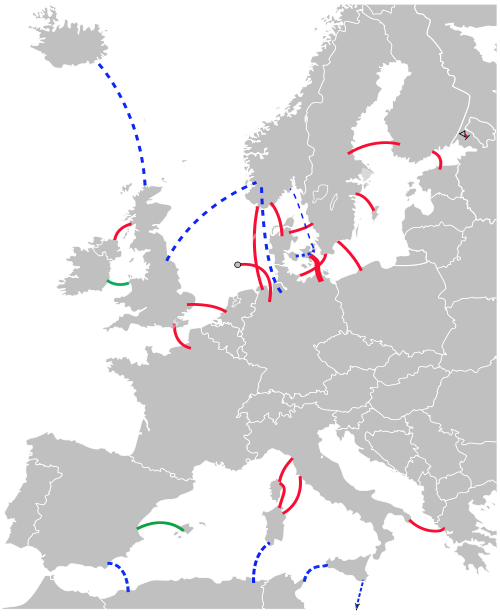
\includegraphics[scale=0.5]{HVDC_Europe.png}
\end{center}
\caption{HGÜ-Leitungen in Europa -- Rot: bestehend, Grün: in Bau; Blau: geplant. Quelle: \cite{Europa}}
\label{pic:Europa}
\end{figure}

In Europa ist der Einsatz von HGÜ jedoch immer noch fast ausschließlich auf Seekabel beschränkt -- auf allen anderen Kontinenten (natürlich ausgenommen der Antarktis) gibt es hingegen auch lange Freileitung.

% mehr Anlagen auflisten?

% Bedeutung für Erneuerbare Energien
